
\section{Motivation}
Compressing a deep learning model into a smaller size typically leads to a smaller model footprint, but it does not always lead to faster
inference time and lower energy consumption. As a motivation example, considering applying \FIXME{four} commonly used model compression
techniques to \FIXME{xx} influential deep learning models -- including \FIXME{xx} \CNNs and \FIXME{RNNs}. Our evaluation platform is a
NVIDIA Jetson TX2 embedded deep learning platform with Tensorflow Mobile \FIXME{v.xx} (see Section~\ref{sec:platform}).

Figure~\ref{} summarizes the change of the storage size, memory footprint, inference time, and energy consumption after applying each model
compression technique.

\ref{fig:motivation}

\begin{figure}[!t]
\centering
\subfloat[][Model size]{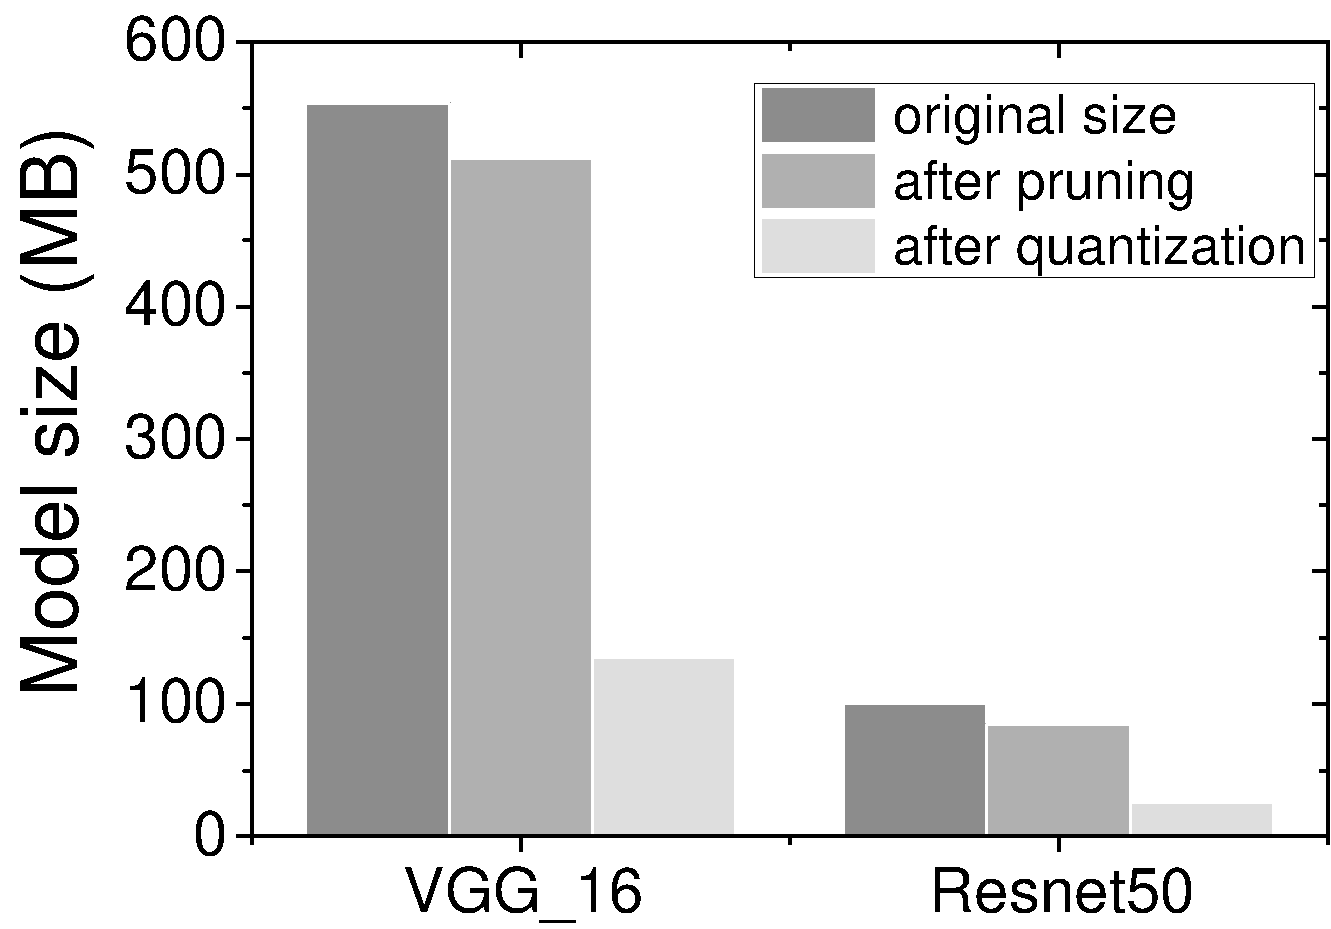
\includegraphics[width=0.4\textwidth]{figure/motivation_size.pdf}}
\hfill
\subfloat[][Inference time]{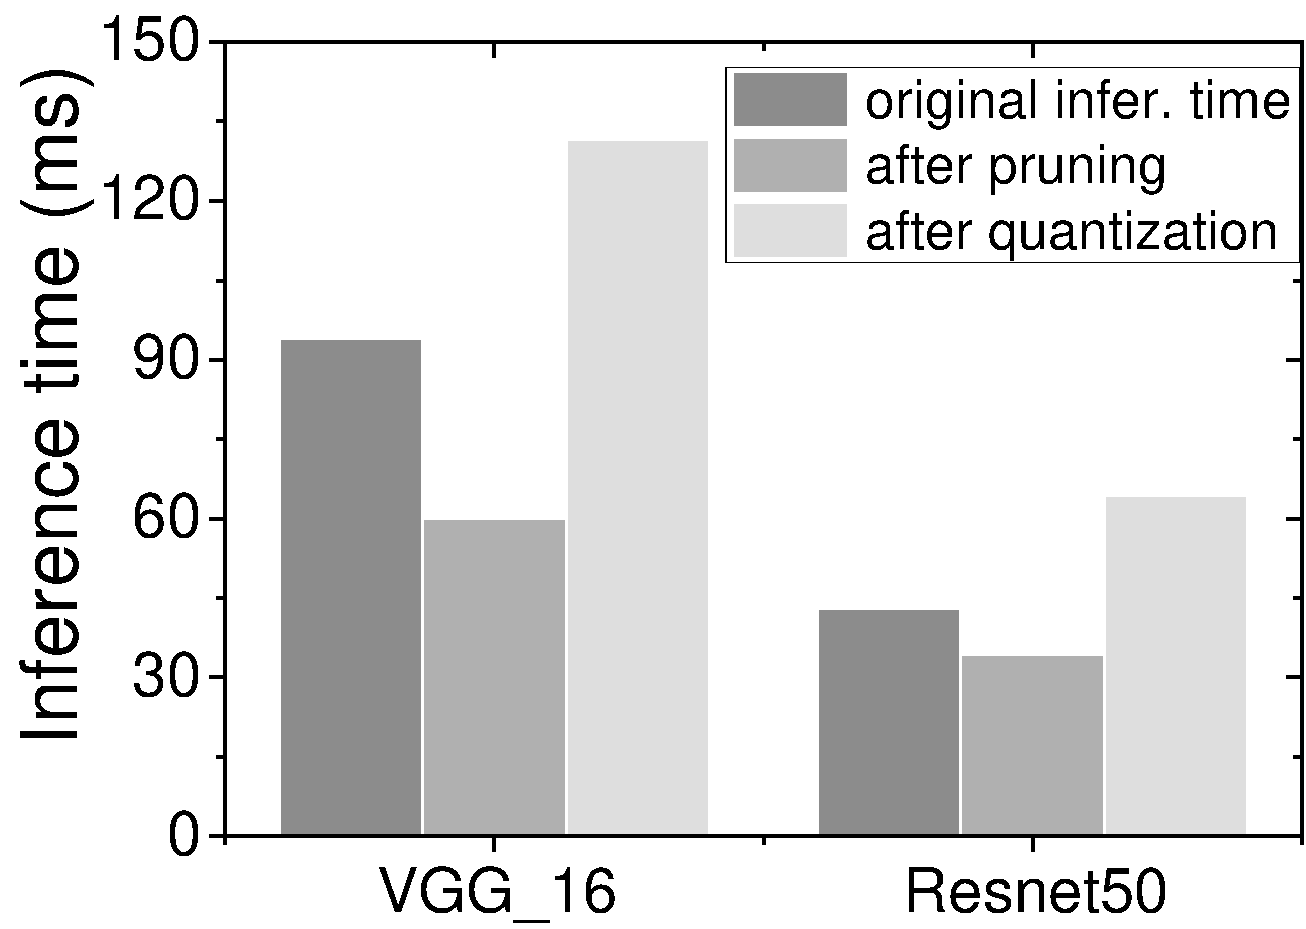
\includegraphics[width=0.4\textwidth]{figure/motivation_time.pdf}}
\caption{The achieved model size (a) and inference time (b) before and after the compression by quantization and pruning.
There is significant room for improvement.}
\label{fig:motivation}
\end{figure}
>>>>>>> origin/master
